\section{Theoretical background}\label{sec:theoretical-background}
The nature of light is a much discussed topic
One view on the matter is that light behaves like a wave as can be seen by the maxwell equations,
one possible solution to the maxwell equations in vacuum is $\vec{E}=\frac{\vec{E_0}}{2}e^{i \left( \vec{k}\cdot\vec{r}-\omega t \right)}+c.c$
and $\vec{B}=\frac{\vec{B_0}}{2}e^{i\left( \vec{k}\cdot\vec{r}-\omega t \right)}+c.c$ where $\|\vec{B_0}\|=\frac{\|\vec{E_0}\|}{c}$ and $\vec{B_0}\bot\vec{E_0}$
which describes a plane wave propagating in the $\vec{k}$ direction.\\
Under this interpretation we expect light to Create an interference pattern when propagating passed a block.\\
To define the shape of the block we shall use an optical transference function (\textbf{OTF}) $T(x,y)$
defined to be 1 where the light is completely unobstructed 0 where no light passes threw and can get any complex value depending on the properties of the block
let us also omit the $+c.c$ from now on.\\
For convenience we shall call the axis perpendicular to our block $z$ and the axes in its plane $x$ and $y$ furthermore we shall call the plane where our wave meets the block
the $z=0$ plane, Thus the wave immediately after the block is expressed by $U_o(x,y,0^-)T(x,y)e^{-i\omega t}$ Where $U_o(x,y,z)$ is the spatial part of the wave function
describing the origin illuminating our block.
We shall mark $\psi(x,y,0,t)=T(x,y)U_o(x,y,0^-)e^{-i\omega t}$ As the wavefunction describing our wave immediately after the block
Such a wavefunction can be described in terms of plane waves as $\psi(\vec{r},t)=\left( \frac{1}{\sqrt{2\pi}} \right)^3 \iiint\limits_{-\infty}^{\quad \infty}b(\vec{k})e^{i \left( \vec{k}\cdot\vec{r}-\omega_k t \right)}d^{3}k$
a further simplification we shall take is to demand that the source will be monochromatic making $\omega_k\rightarrow \omega_0$ $\omega_0=k_{0}c=\|\vec{k}\|c \Rightarrow k_z=\sqrt{k_0^2-k_x^2-k_y^2}$
And thus our 3 dimensional integral is reduced to 2 dimensions:
\begin{aligned}
    &\psi\rightarrow\hat{\psi}=\frac{1}{\sqrt{2\pi}^3}e^{-i\omega_0 t}\underbrace{\iint\limits_{-\infty}^{\quad \infty}
    b(\vec{k})e^{i\left( k_x x+k_y y+\sqrt{k_0^2 -k_x^2 -k_y^2} z \right)}dk_x dk_y}_{U(x,y,z)}\\
    &\Rightarrow U_o(x,y,0^-)T(x,y)=\frac{1}{\sqrt{2\pi}^3} \iint \limits_{-\infty}^{\quad \infty}b(k_x,k_y)e^{ik_x x+k_y y}= \\
    &\frac{\mathcal{FT}^{-1}\left[ b(k_x,k_y) \right]}{\sqrt{2\pi}}\Rightarrow b(k_x,k_y)=\sqrt{2\pi} \mathcal{FT}_{2D}\left[ U(x,y,0)
    \right]
\end{aligned}
\\Summarizing, we have:\\
$\psi(\vec{r},t)=\frac{1}{2\pi} \iint\limits_{-\infty}^{\quad \infty}\mathcal{FT}\left[ T(x,y)U_o(x,y,0^-) \right]e^{i \left( \vec{k}\cdot\vec{r}-\omega_0 t \right)}dk_x dk_y$
under the approximation where $|k_x|,|k_y| \ll \|\vec{k}\|$ we get:
\begin{align} \label{eq:nearfield}
    &U(\vec{r})=\frac{k_0 e^{ik_0 z}}{2\pi iz}\iint\limits_{-\infty}^{\quad \infty}U(x',y',0)e^{i\frac{k_0}{2z}((x-x')^2+(y-y'^2))}dx' dy'
\end{align}
known as the Fresnel integral\cite{fresnel}.\\
Taking the approximation further and assuming also $\frac{k_0 D^2}{2z} \ll \pi$ where $D$ is a length such that T(x,y) is 0 outside a square of side length $D$
we get:
\begin{equation}\label{eq:farfield}
    U(x,y,z)=-\frac{ik}{z}e^{ik(z+\frac{x^2+y^2}{2z})}\mathcal{FT}\left[ U(x',y',0) \right]\\
    _{k_x=\frac{kx}{z},k_y=\frac{ky}{z}}
\end{equation}
known as the far field approximation.\\
Finally let us define as $I=|U|^2$ The reason for this definition is that our measuring devices measures a time average of the amplitude of our wave function $\psi$.\\
Our final subject is the case where the slit is of a shape as in~\ref{fig:expansion slit shape}, for a spring such as in~\ref{fig:spring parameters illustration}
the interference pattern is as shown in~\ref{fig:expansion interference simulation} notice the "X" shape with angle $\theta$ between the arms of the "X"
this angle is indeed half of the angle $2\theta$ shown in~\ref{fig:spring parameters illustration}
as for the arms themselves notice the interference within them, the spacing between maxima in the two arms slightly differs,
let us mark $\Delta_1$ as the smaller of the two and $\Delta_2$ as the larger.
now the diameter of the spring can be calculated as
$d=\frac{\lambda z}{\Delta_1}$ and the pitch as $p=\frac{\lambda z}{\Delta_2 \cos \theta}$.\\
\begin{figure}[H]
    \centering
    \begin{subfigure}{0.48\columnwidth}
        \centering
        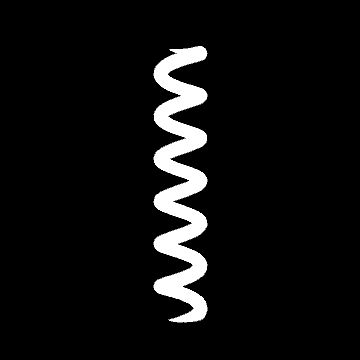
\includegraphics[width=\columnwidth]{figures/slit shape.png} % first figure itself
        \caption{slit shape of a helix generated by projecting a 3d helix on to a plane}
        \label{fig:expansion slit shape}
    \end{subfigure}\hfill
    \begin{subfigure}{0.48\columnwidth}
        \centering
        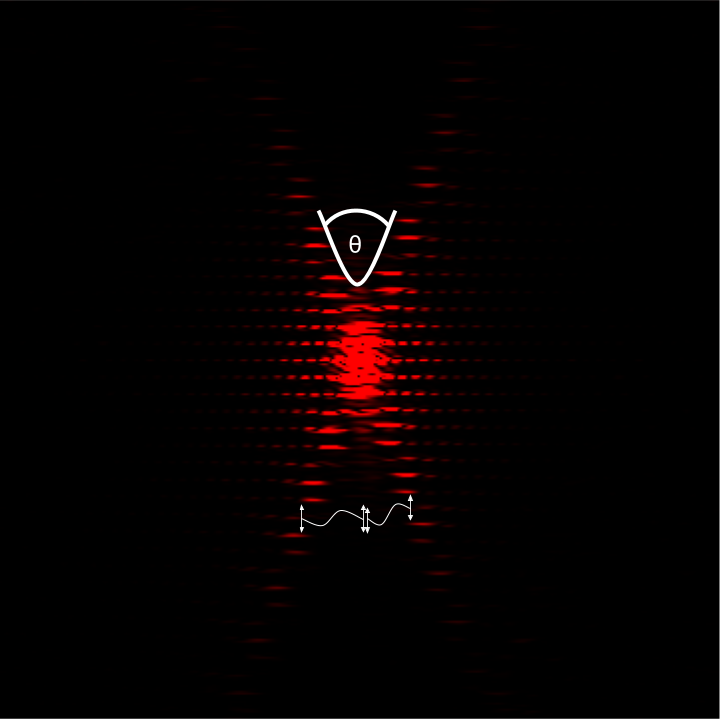
\includegraphics[width=\columnwidth]{figures/interference pattern.png} % second figure itself
        \caption{magnitude square of discrete fourie transform of slit shape shown in \ref{fig:expansion slit shape}}
        \label{fig:expansion interference simulation}
    \end{subfigure}
    \begin{subfigure}{0.48\columnwidth}
        \centering
        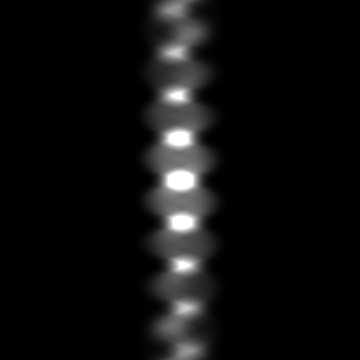
\includegraphics[width=\columnwidth]{figures/reverse fourie transform.png}
        \caption{inverse fourie transform of \ref{fig:expansion interference simulation} showing
        the inverse fourie transform of the square of the fourie transform of \ref{fig:expansion slit shape}}
        \label{fig:expansion inverse fourie transform}
    \end{subfigure}
    \begin{subfigure}{0.48\columnwidth}
        \centering
        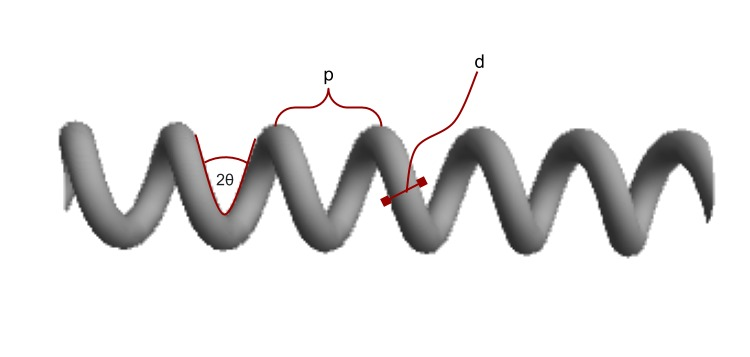
\includegraphics[width=\columnwidth]{figures/spring parameters illustration.jpg}
        \caption{spring parameters illustration}
        \label{fig:spring parameters illustration}
    \end{subfigure}

    \label{fig:expansion theory illustrations}
\end{figure}

Another principle we rely on is Babinet's principle\cite{babinet} which states that the diffraction pattern of some diffracting body $B$ is identical to its optical complement $B'$ up to a multiplicative factor.
An optical complement of some object is defined to be opaque where the original body is transparent and vice versa.